
\documentclass[12pt]{article}
\usepackage{amsmath}
\usepackage{url}
\usepackage{multirow}
\usepackage{array}
\newcolumntype{N}{>{\centering\arraybackslash}m{.5in}}
\usepackage{lscape}
\usepackage{graphicx}
\usepackage{setspace}
\usepackage{float}
\usepackage[sort&compress]{natbib}
\usepackage[labelfont=bf]{caption}
% \usepackage[pagewise]{lineno} %command for numberling lines. It needs file ``lineno.sty''

% The following parameters seem to provide a reasonable page setup.
\topmargin 0.0cm
\oddsidemargin 0.2cm
\textwidth 16cm
\textheight 21cm
\footskip 1.0cm
\doublespacing

\title{Supporting Infomation }
\author{Cervantes-Loreto et al.}
\date{}

\begin{document}
\maketitle
\renewcommand{\thesection}{S\arabic{section}}
\renewcommand{\thefigure}{S\arabic{figure}}
\renewcommand{\thetable}{S\arabic{table}}
\renewcommand{\theequation}{S\arabic{equation}}





\begin{figure}[H]
  \centerline{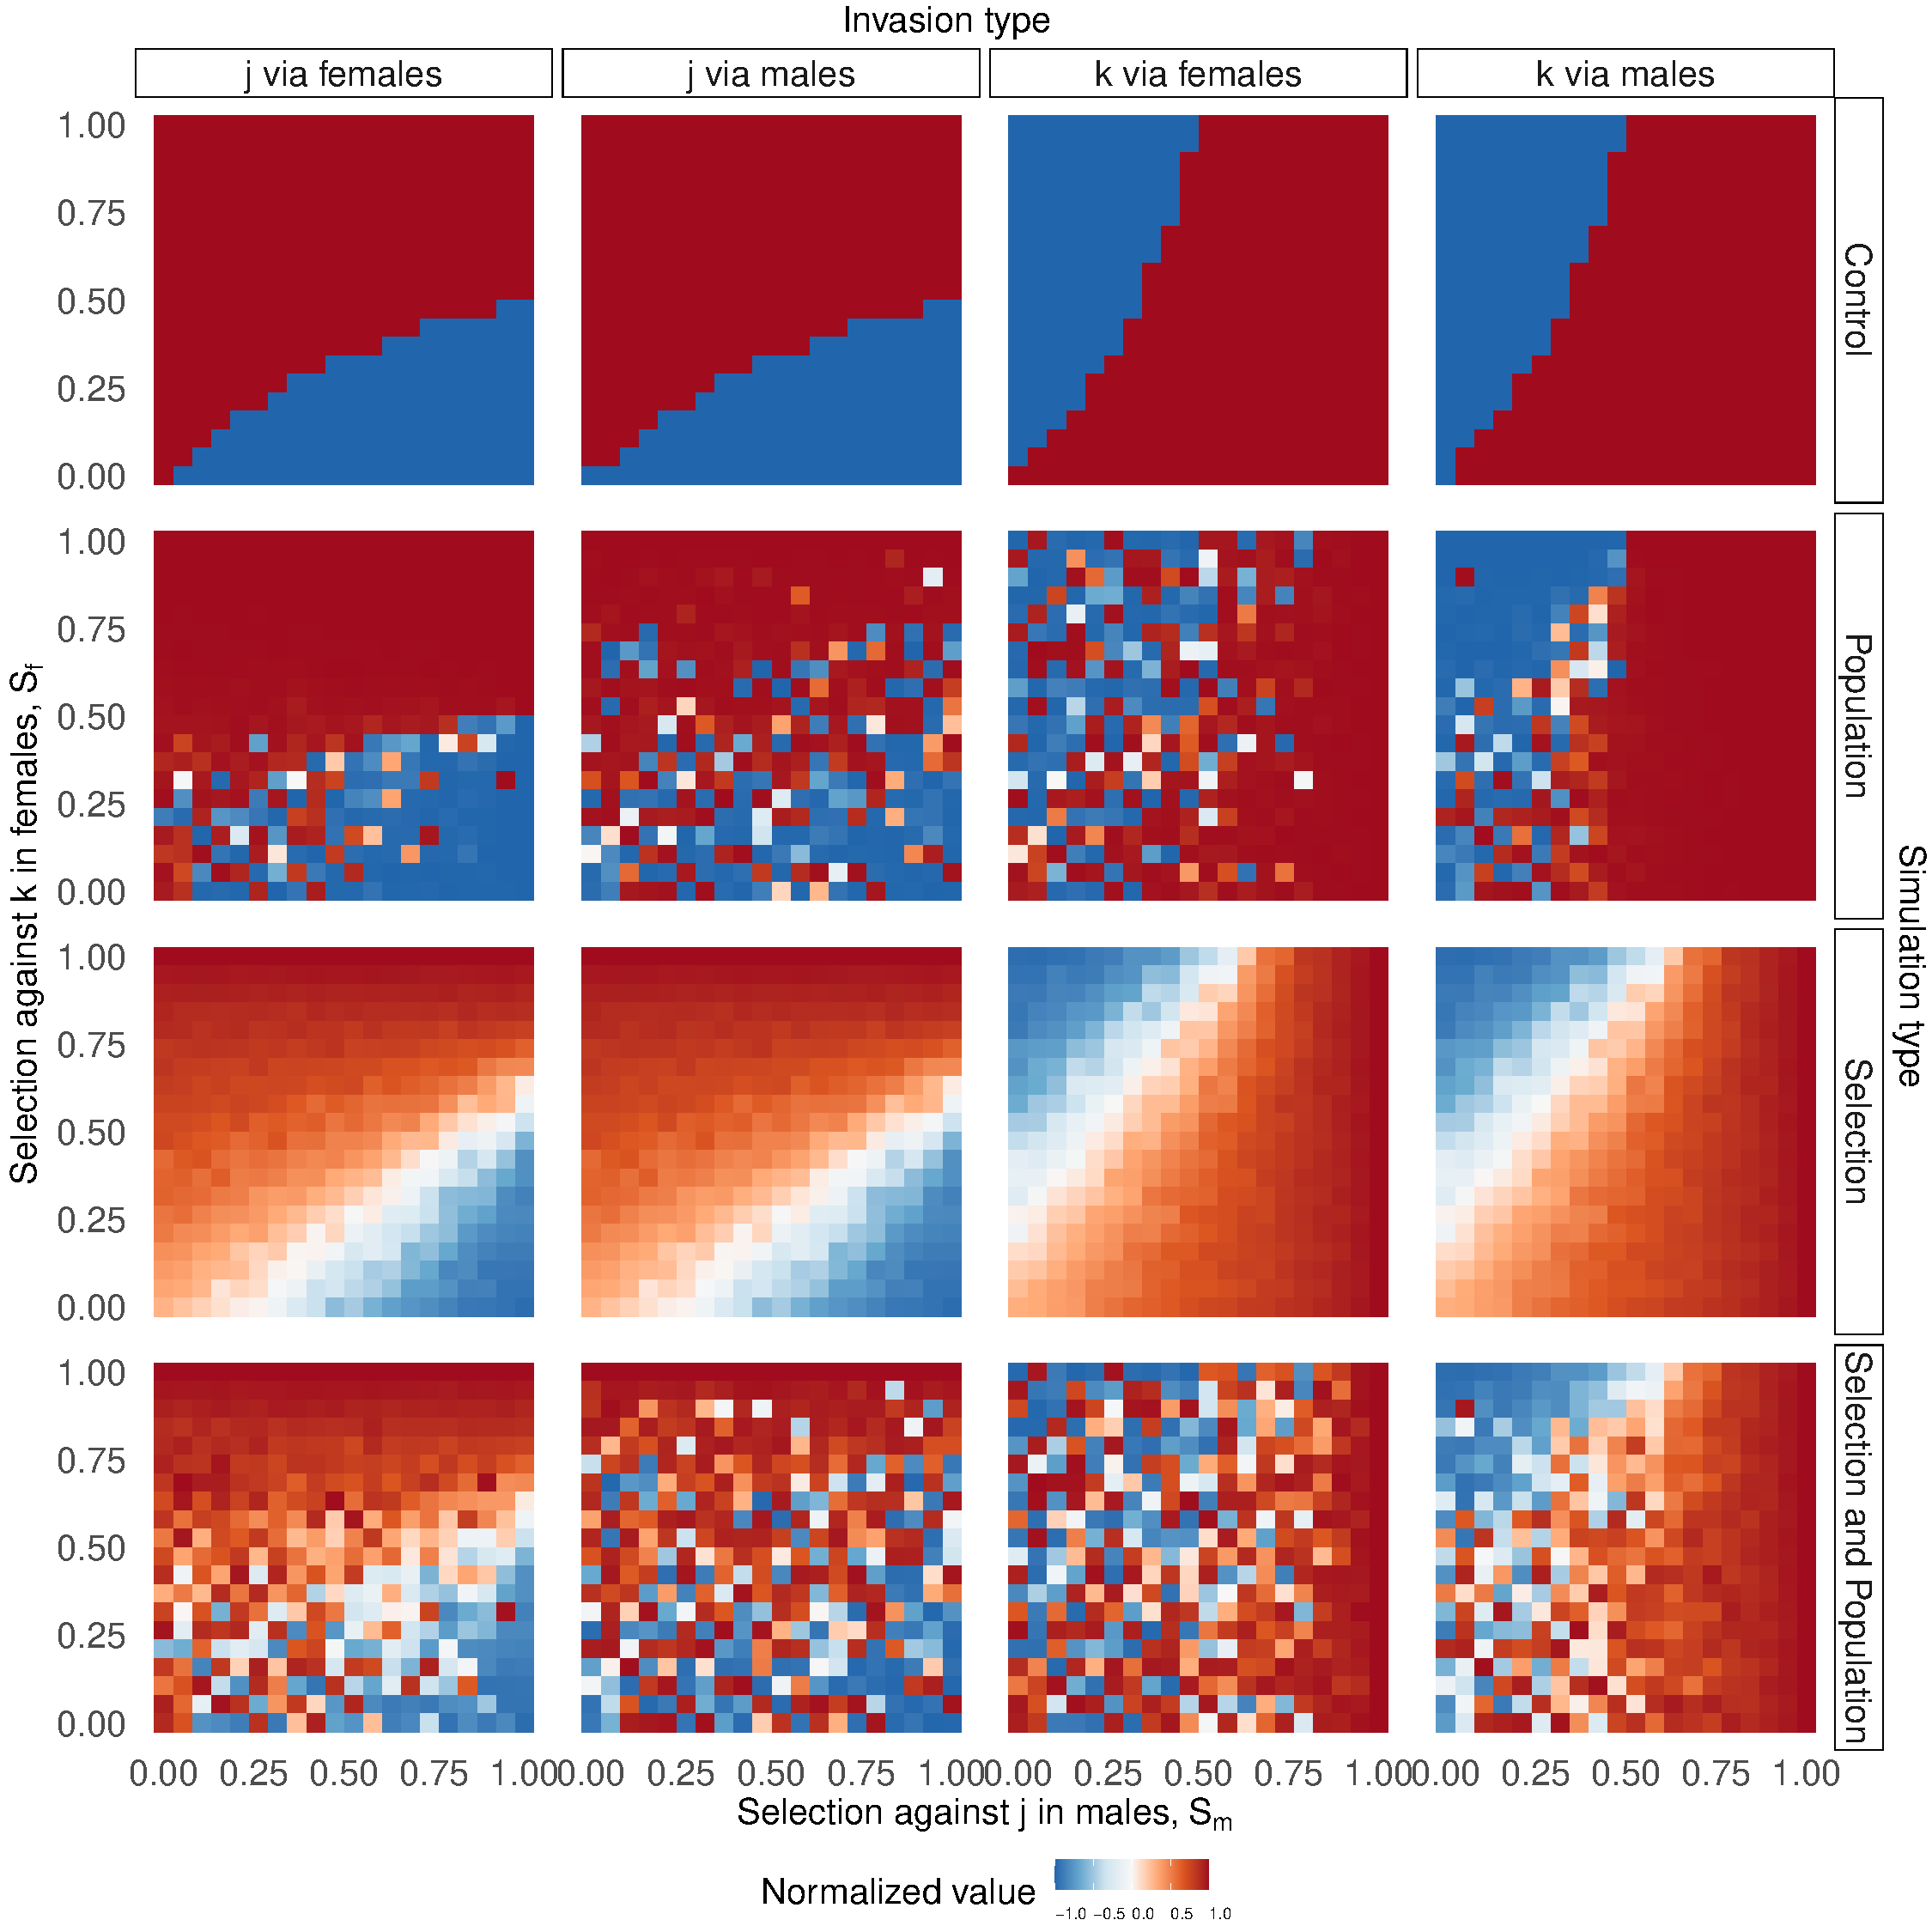
\includegraphics[width=1\textwidth]{ratios.pdf}}
  \caption{ The normalized value of  $\delta^{0}$ in the selection parameter space. Each row in this figure corresponds to one replicate of a different type of simulation, while each column corresponds to a different type of invasion. In the Control simulation ($\sigma_{g}=0.001$, $\rho_{g}=0$, $\sigma_{w}=0.001$, $\rho_{w}=0$), $\delta^{0}$ had a normalized value of 1 in parts of the parameter space where selection allows each allele to be fixed in a population, and a value of -1 where each allele can not be mantained in a population. The Population simulation corresponds to a replicate of a simulation where only population sizes fluctuated, without correlation between fluctuations ($\sigma_{g}=70$, $\rho_{g}=0$, $\sigma_{w}=0.001$, $\rho_{w}=0$). The Selection simulation corresponds to a replicate of a simulation where only selection fluctuated, without correlations betweeen fluctuations ($\sigma_{g}=0.001$, $\rho_{g}=0$, $\sigma_{w}=0.9$, $\rho_{w}=0$). Finally, the Selection Population simulation corresponds to a replicate of a simulation where both selection and population sizes fluctuated, without correlations between fluctuations ($\sigma_{g}=70$, $\rho_{g}=0$, $\sigma_{w}=0.9$, $\rho_{w}=0$).  }
    \label{fig:ratios}
\end{figure}

\clearpage
\begin{figure}[H]
  \centerline{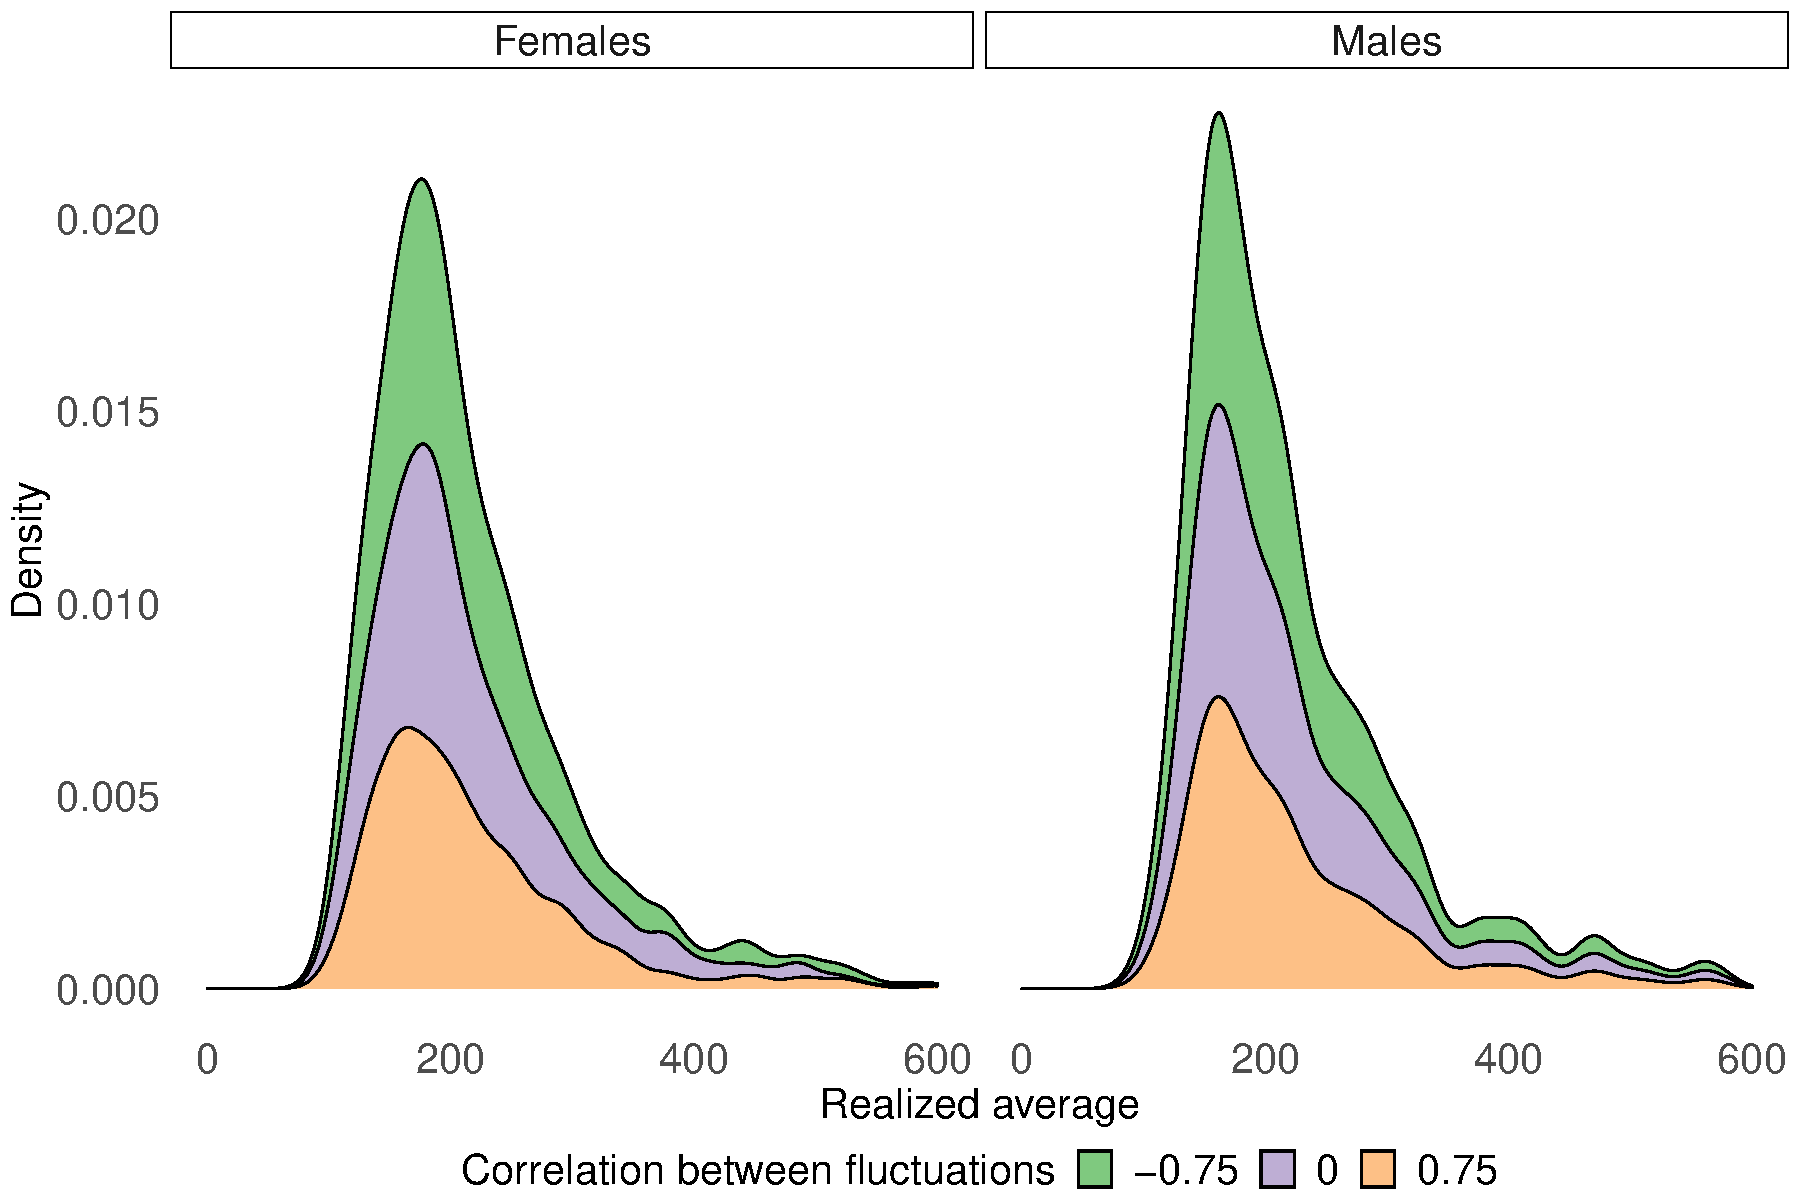
\includegraphics[width=0.8\textwidth]{realized_average.pdf}}
  \caption{ Distributions of mean population sizes in three simulations. Without fluctuations, the mean population size for each sex was 200 individuals. However, when we incorporated large fluctuations in population sizes the mean population size for each sex ranged from $\approx 100$ individuals to $\approx 600$. To exemplify this, we show for three simulations where only population sizes fluctuated ($\sigma_{g}=70$, $\sigma_{w}=0.001$, $\rho_{w}=0$), the distribution of realized mean population sizes across the selection parameter space. Each row corresponds to a different correlation between fluctuations, and each column to a different sex.  }

\end{figure}

\clearpage

\begin{figure}[H]
  \centerline{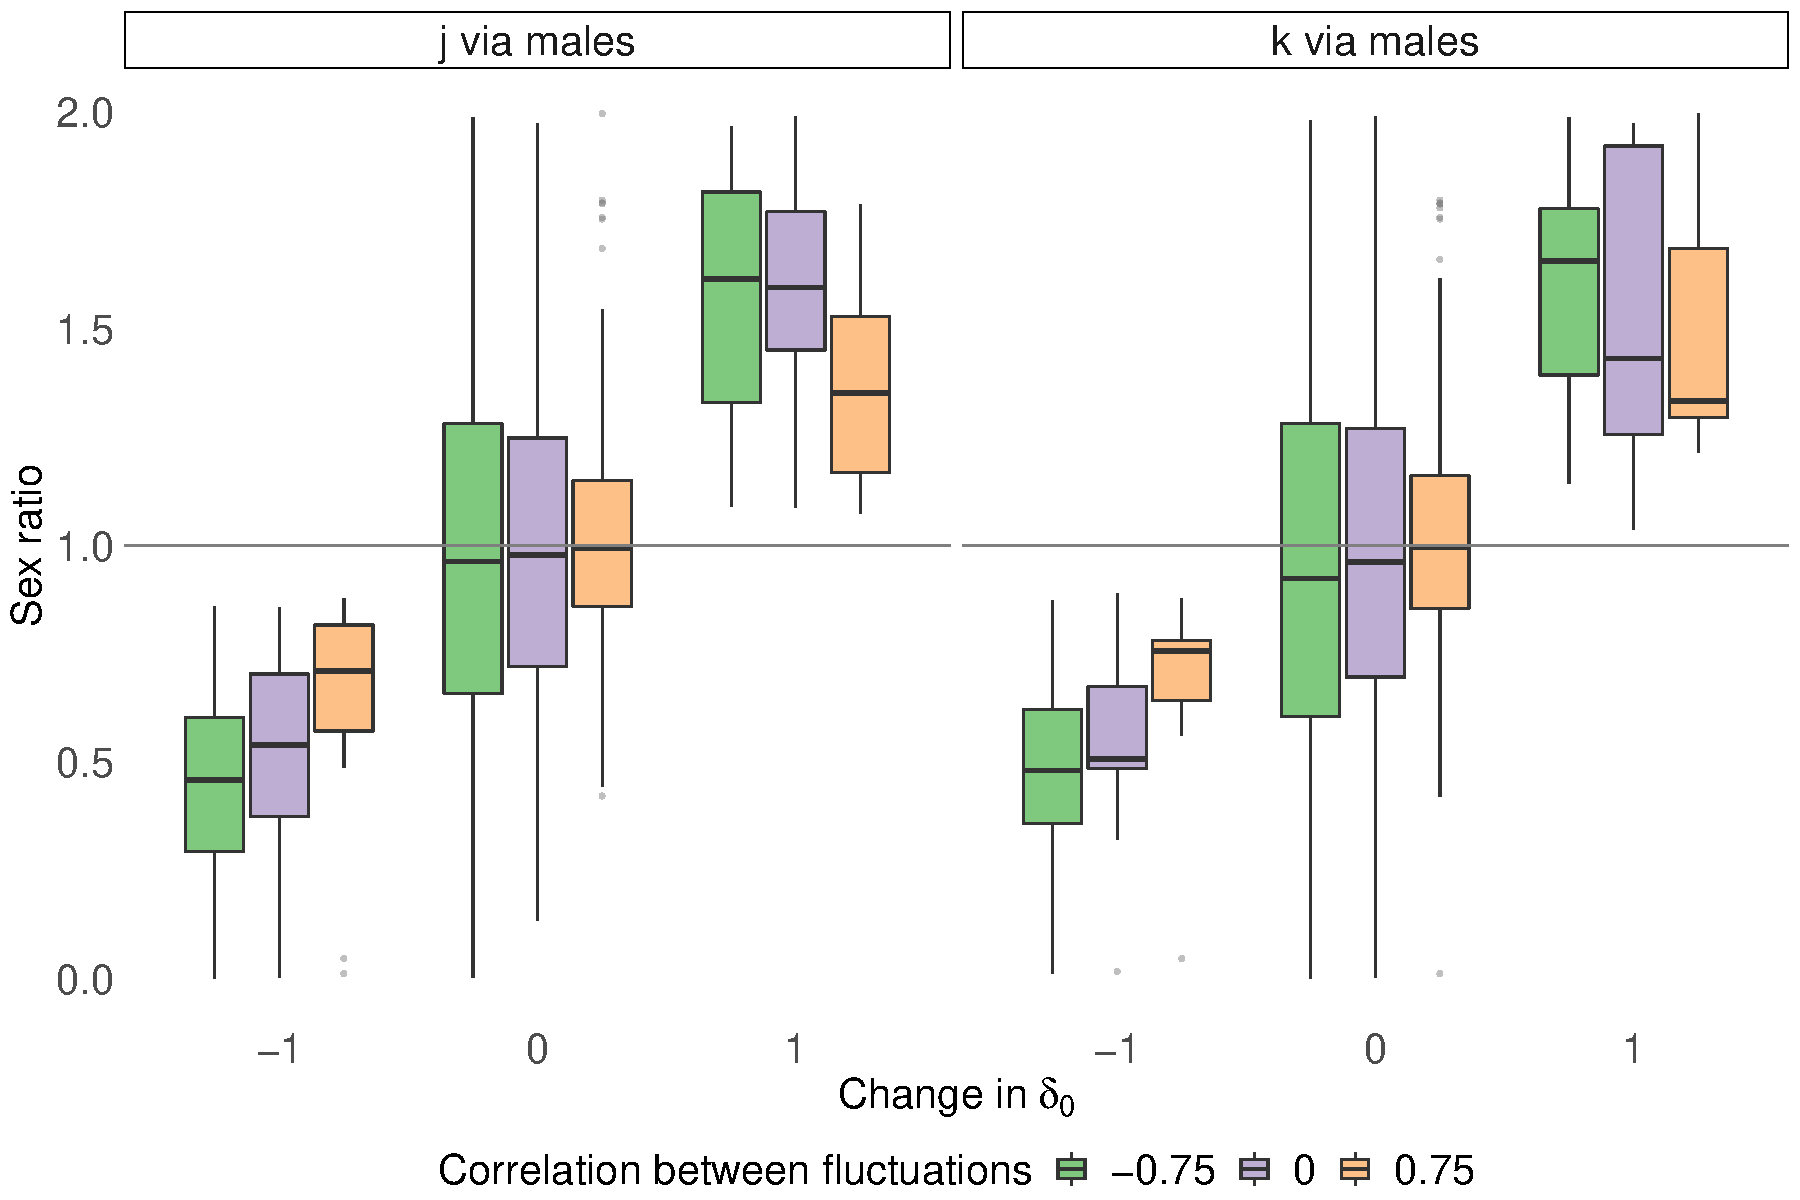
\includegraphics[width=0.8\textwidth]{males.pdf}}
  \caption{ Changes to $\delta_{0}$ and sex ratios when males invade. For all of the replicates of simulations with large fluctuations of population sizes ($\sigma_{g}=70$, $\sigma_{w}=0.001$, $\rho_{w}=0$), we show how changes in the value of  $\delta_{0}$ compared to the control simulation were associated to skewed sex ratios when alleles invaded via males. Each panel shows the results for a different allele invading.  We qualitatively grouped changes across the selection parameter space of each simulation as -1 if $\delta_{0}$ was positive in the control simulation but changed to negative in the examined simulation, as 1 if $\delta_{0}$ was negative in the control simulation but changed to positive in the examined simulation, and 0 if the sign of delta remained the same. We also calculated the sex ratio when populations were set to their means in each part of the parameter space of each simulation. We calculated the sex ratio as $\frac{N_{f}}{N_{m}}$ and thus values greater than 1 indicate the population has more females than males, while values less than 1 indicate populations with more males than females. We show different correlations between fluctuations in the examined simulations with different colors, as the legend describes. Box plots extend from the first to third quantiles of the corresponding posterior distribution of parameter values, and the line inside the box indicates the median. The upper whisker extends to the largest value no further than 1.5 times the inter-quantile range (IQR, or the distance between the first and third quartiles); the lower whisker extends to the smallest value at most 1.5 times the IQR. Data beyond the end of the whiskers are determined to be outliers and are plotted individually with solid grey points }

\end{figure}

\clearpage

\begin{figure}[H]
  \centerline{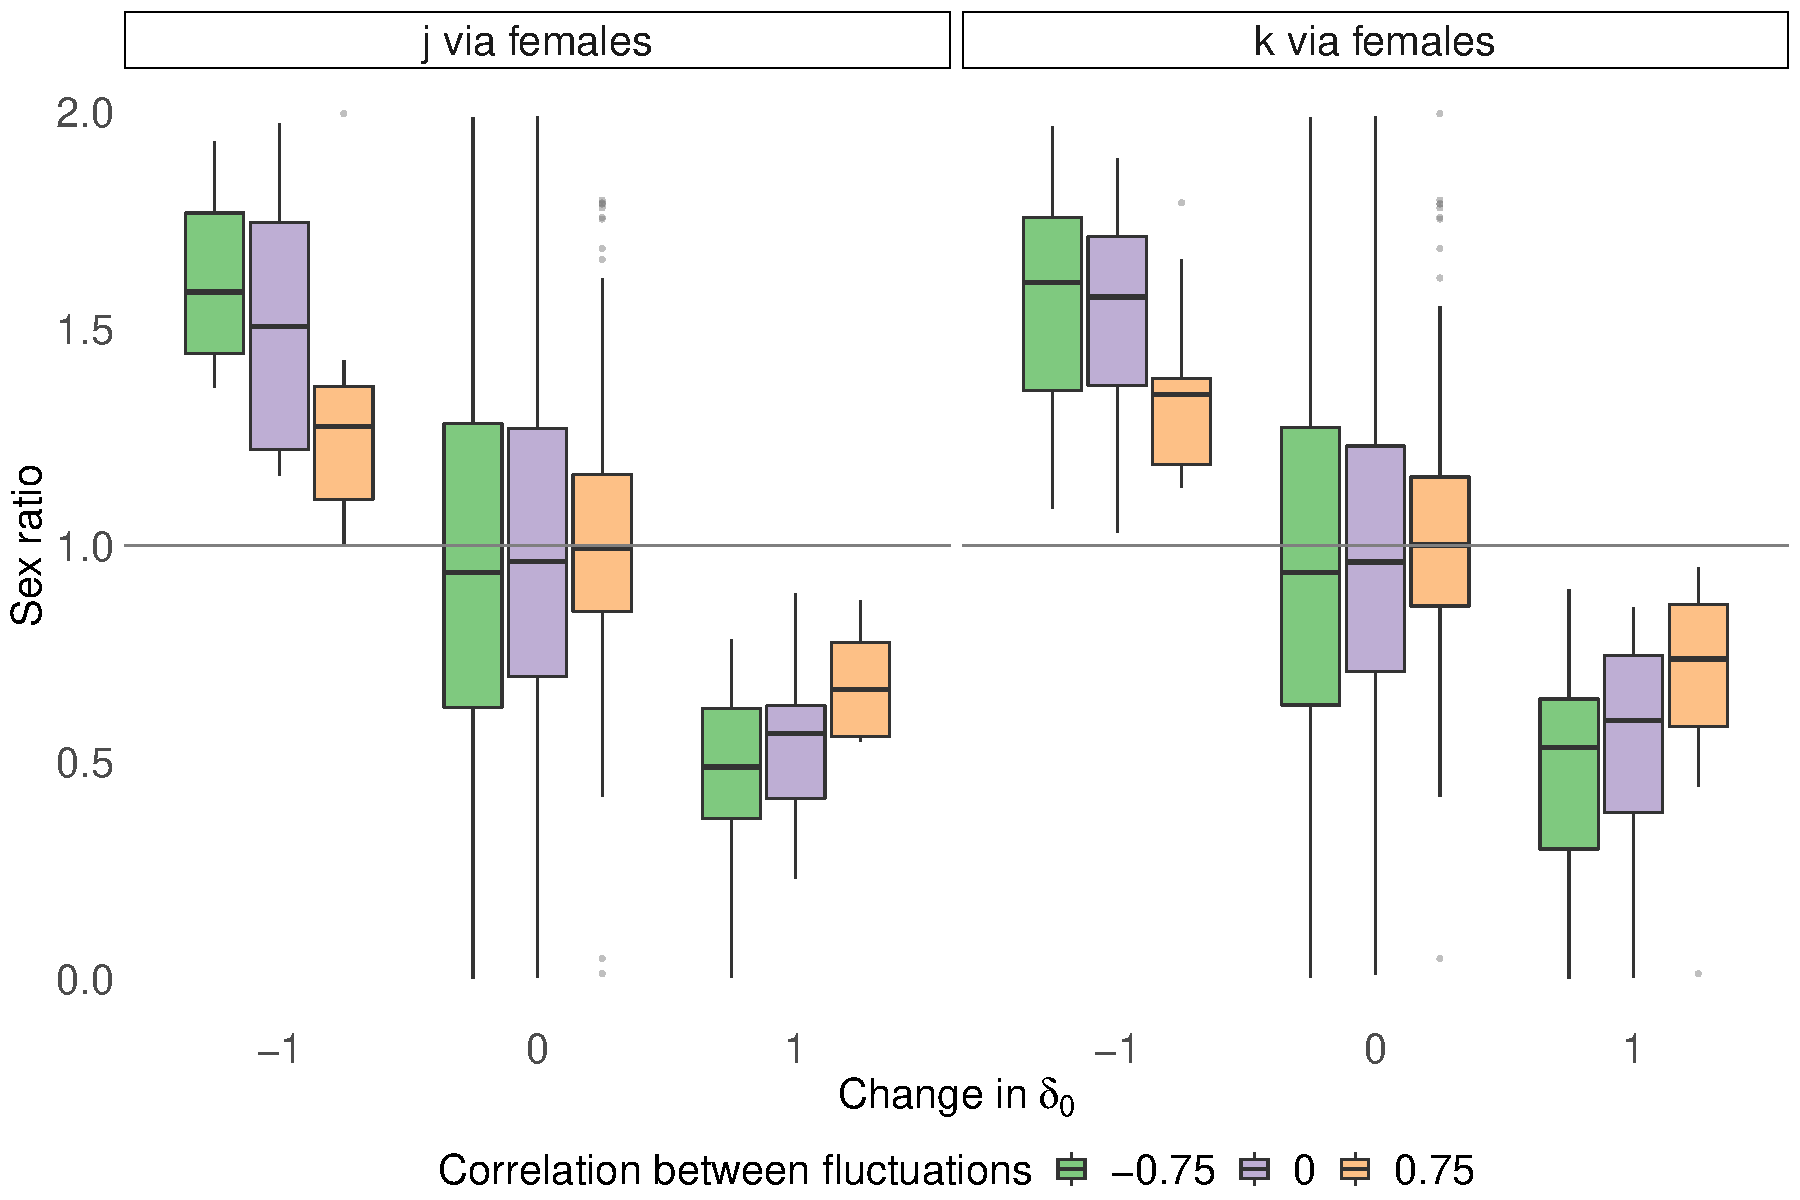
\includegraphics[width=0.8\textwidth]{females.pdf}}
  \caption{Changes to $\delta_{0}$ and sex ratios when females invade. For all of the replicates of simulations with large fluctuations of population sizes ($\sigma_{g}=70$, $\sigma_{w}=0.001$, $\rho_{w}=0$), we show how changes in the value of  $\delta_{0}$ compared to the control simulation were associated to skewed sex ratios when alleles invaded via females. Each panel shows the results for a different allele invading.  We qualitatively grouped changes across the selection parameter space of each simulation as -1 if $\delta_{0}$ was positive in the control simulation but changed to negative in the examined simulation, as 1 if $\delta_{0}$ was negative in the control simulation but changed to positive in the examined simulation, and 0 if the sign of delta remained the same. We also calculated the sex ratio when populations were set to their means in each part of the parameter space of each simulation. We calculated the sex ratio as $\frac{N_{f}}{N_{m}}$ and thus values greater than 1 indicate the population has more females than males, while values less than 1 indicate populations with more males than females. We show different correlations between fluctuations in the examined simulations with different colors, as the legend describes. Box plots extend from the first to third quantiles of the corresponding posterior distribution of parameter values, and the line inside the box indicates the median. The upper whisker extends to the largest value no further than 1.5 times the inter-quantile range (IQR, or the distance between the first and third quartiles); the lower whisker extends to the smallest value at most 1.5 times the IQR. Data beyond the end of the whiskers are determined to be outliers and are plotted individually with solid grey points }

\end{figure}




%\bibliographystyle{ecology_letters}
%\bibliography{references.bib}

\end{document}
